\section{Exact string joins with taxonomy}

We consider the exact joins including hypernymy and hyponymy and mixed three predicates based on taxonomy T.

The baseline join algorithm is the nested-loop join. All string pairs are accessed to determine the hyper-hypo relationships. But this algorithm is obviously not efficient. Therefore, we propose an efficient algorithm.



\begin{figure}[t]
\centering
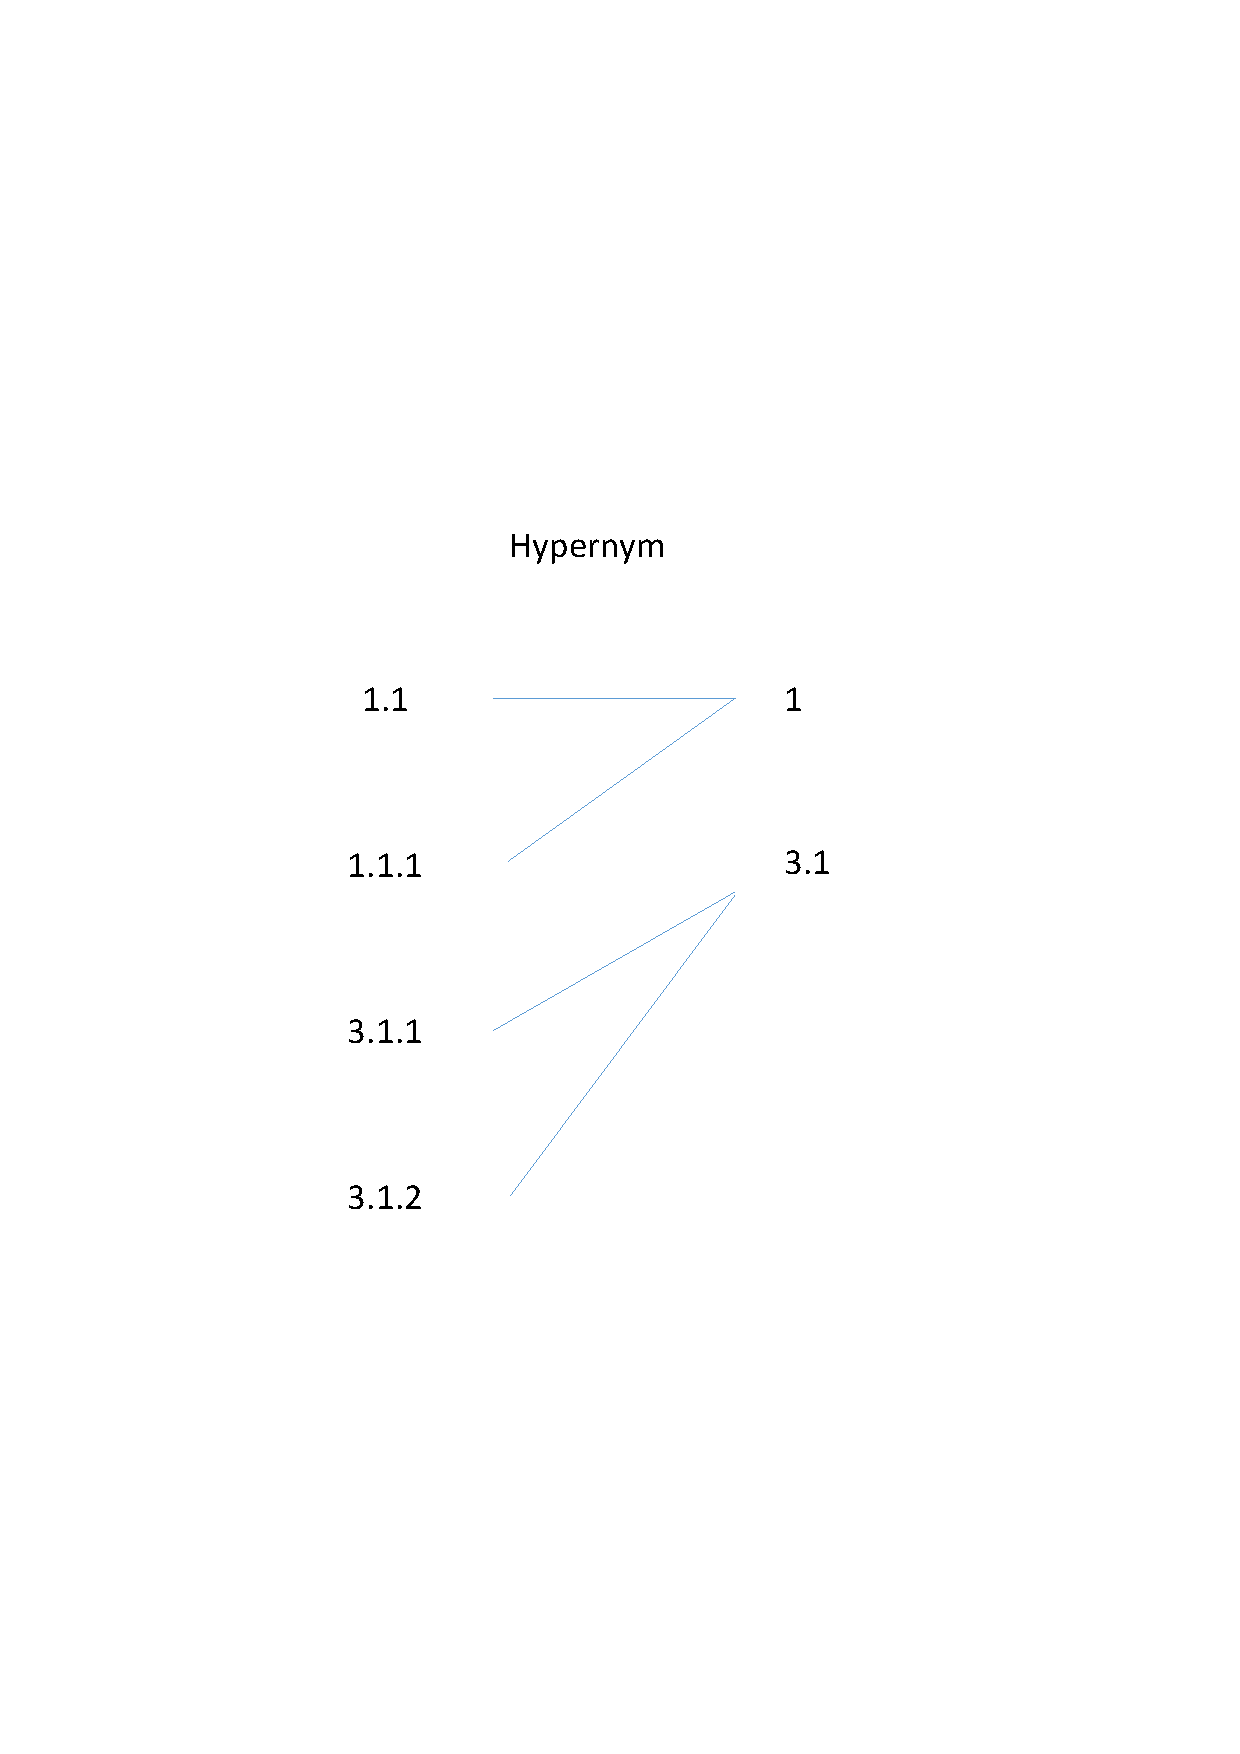
\includegraphics[scale=0.4]{figures/labeljoins}
 \caption{Join inverted lists}
\label{fig:taxonomy}
\end{figure}


%\begin{algorithm}
%{\bf Input}: two strings $s_1$ and $s_2$ \\
%{\bf Output}: four relationships: R=\{Hype, Hypo, Equa and Non\}
%\begin{compactenum}[(1)]
%\item {\bf If} ($s_1 = s_2$ )  {\bf return} Equa;
%\item {\bf If} ($|LCD(s_1)| >$ 1 AND $|LCD(s_2)| >$ 1 )  {\bf return} None;
%\item {\bf Else} {\bf if} ($|LCD(s_1)| =$ 1 AND $|LCD(s_2)| >$ 1 )
%\item \verb"  " {\bf If}  $\forall t \in LCD(s_1)$, $t$ is a hypernym of $LCD(s_2)$
%\item \verb"    " {\bf return} Hype {\bf else} {\bf return} None;
%\item {\bf Else} {\bf if} ($|LCD(s_2)| =$ 1 AND $|LCD(s_1)| >$ 1 )
%\item \verb"  " {\bf If}  $\forall t \in LCD(s_2)$, $t$ is a hypernym of $LCD(s_1)$
%\item  \verb"    " {\bf return} Hypo {\bf else} {\bf return} None;
%\item {\bf Else} /\ *  $|LCD(s_1)| = |LCD(s_2)| = $ 1 */\
%\item  \verb"  " {\bf If}  $LCD(s_1)$ is a hypernym of $LCD(s_2)$  {\bf return} Hype
%\item   \verb"  " {\bf Else if}  $LCD(s_1)$ is a hyponym of $LCD(s_2)$  {\bf return} Hypo
%\item   \verb"  " {\bf Else return} none
%\end{compactenum}
%\caption{Determine the relationship between two strings}
%\label{alg:measure}
%\end{algorithm}


\begin{algorithm}
{\bf Input}: two sets of strings $S_1$ and $S_2$, a taxonomy $T$ \\
{\bf Output}: string pairs $(s_1,s_2) \in S_1 \times S_2$ s.t. $s_1 \sqsubset s_2$ or $s_2 \sqsubset s_1$
\begin{compactenum}[(1)]
\item Let $G_s$ and $G_t$ denote the inverted lists for S and T respectively.
\item Perform a join operation to find the IS-A relationship between $G_s$ and $G_t$
\item {\bf FOR} EACH join pair ($t_1,t_2$)
\item  $R = R \cup t_1.List \times t_2.List$
\item $R$
\end{compactenum}
\caption{String joins with taxonomy}
\label{alg:exactjoin}
\end{algorithm}

Note that the above algorithm may contain the duplicate result set. Therefore, we need to sort and remove the duplication.



\subsection{Join algorithms}

The key to an efficient, uniform mechanism for set-at-atime
(join-based) matching of query graph patterns is a positional
representation of occurrences of  elements and in the taxonomy database (see, e.g., [6, 7, 27]),
which extends the classic inverted index data structure in information retrieval [22]. We borrow the labeling scheme from XML databases and use the prefix based labels. Structural relationships between tree nodes whose positions
are recorded in this fashion can be determined easily for hypernym or hyponym relationships.

There are two kinds of edges in a graph pattern, ``$\rightarrow$'' and ``$\leftarrow$''shows the IS-A relationship, hypernym and hyponym and ``$\leftrightarrows$'' is a mixedISA relationship.

In general, at each node in the query graph pattern, there is
a node predicate on the attributes (e.g., tag, content) of the
node in question. For the purposes of this paper, exactly
what is permitted in this predicate is not material.  It suffices
for our purposes that there be efficient access mechanisms
(such as index structures) to identify the nodes in the
database that satisfy any given node predicate $q$, and
return a stream of matches $T_q$ based on the taxonomy.

\begin{theorem}  Algorithm \ref{alg:exactjoin} is an optimal algorithm. The computing cost is linear to the sum of the size of the input and output. That is, each output result contribute to the final answer.
\end{theorem}



